\documentclass[tikz,border=8pt]{standalone}
\usetikzlibrary{arrows.meta,positioning}
\begin{document}
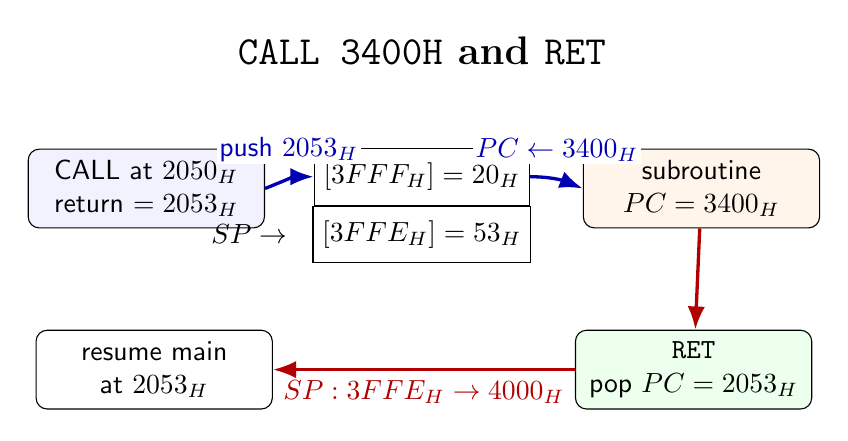
\begin{tikzpicture}[font=\sffamily,>=Latex,box/.style={draw,rounded corners,minimum width=3.0cm,minimum height=1cm,align=center},mem/.style={draw,minimum width=2.5cm,minimum height=.72cm}]
\node[font=\Large\bfseries] at (5.2,5.25) {\texttt{CALL 3400H} and \texttt{RET}};
\node[box,fill=blue!5] (call) at (1.7,3.5) {CALL at $2050_H$\\return $=2053_H$};
\node[box,fill=orange!8] (sub) at (8.75,3.5) {subroutine\\$PC=3400_H$};
\node[mem] (mh) at (5.2,3.65) {$[3FFF_H]=20_H$};
\node[mem,below=0pt of mh] (ml) {$[3FFE_H]=53_H$};
\node[left=2mm of ml] {$SP\to$};
\draw[very thick,blue!70!black,->] (call.east) to[out=22,in=180]
  node[midway,above=5pt,fill=white,inner sep=1pt] {push $2053_H$} (mh.west);
\draw[very thick,blue!70!black,->] (mh.east) to[out=0,in=158]
  node[midway,above=5pt,fill=white,inner sep=1pt] {$PC\leftarrow3400_H$} (sub.west);
\node[box,fill=green!7] (ret) at (8.65,1.2) {\texttt{RET}\\pop $PC=2053_H$};
\node[box] (resume) at (1.8,1.2) {resume main\\at $2053_H$};
\draw[very thick,red!70!black,->] (sub)--(ret);
\draw[very thick,red!70!black,->] (ret)--(resume) node[midway,below] {$SP:3FFE_H\to4000_H$};
\end{tikzpicture}
\end{document}
